\section{Waves}
\subsection{General properties of waves}

\begin{point}
Know that waves transfer energy without transferring matter
\end{point}

\begin{point}
Describe what is meant by wave motion as illustrated by vibrations in ropes and springs and by experiments 
using water waves
\end{point}

The waves themselves never move. The particles that make up the wave oscillate, (move periodically
back and forth) without movement of the wave itself. This can be illustrated by the movements
of a rope, when one end is moved up and down periodically. In case of a spring, forward and
backward movements at one end of a spring compress and expand parts of the spring, these parts
move along the spring, which is wave movement.

\begin{point}
Describe the features of a wave in terms of wavefront, wavelength, frequency, crest (peak), trough, 
amplitude and wave speed
\end{point}

The wave crests and troughs of multiple parallel waves form lines, called \ul{\emph{wavefronts}}. 

The wavelength, frequency and amplitude are defined in following subsections.

The \ul{\emph{crest}} is the maximum displacement of a particle in a wave.
The \ul{\emph{trough}} is the minimum displacement of a particle in a wave.

\begin{figure}
	\centering
	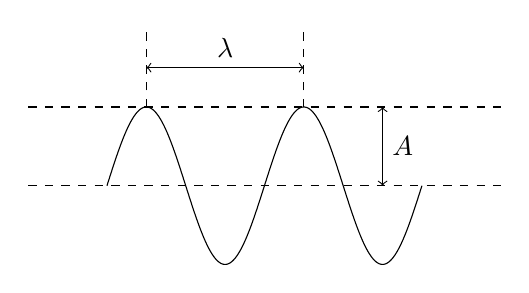
\begin{tikzpicture}
		% Draw sine wave
		\draw[domain=0:720, samples=200, smooth] plot ({\x/360*2}, {sin(\x)});
		\draw[dashed] (-1, 0) -- (5, 0);

		\draw[<->] (0.5, 1.5) -- (2.5, 1.5) node[midway, above]{$\lambda$};
		\draw[dashed] (0.5, 1) -- (0.5, 2);
		\draw[dashed] (2.5, 1) -- (2.5, 2);

		\draw[dashed] (-1, 1) -- (5, 1);
		\draw[<->] (3.5, 0) -- (3.5, 1) node[midway, right]{$A$};
	\end{tikzpicture}
	\caption{A wave}
\end{figure}

\begin{point}
Define the terms:
\begin{enumerate}[label=(\alph*)]
	\setlength\itemsep{0em}
	\item frequency as the number of wavelengths that pass a point per unit time
	\item wavelength as the distance between two consecutive, identical points such as two consecutive crests
	\item amplitude as the maximum distance from the mean position
\end{enumerate}
\end{point}

The \ul{\emph{wavelength}} and \ul{\emph{amplitude}} are shown in Figure 7 as $\lambda$ and
$A$, respectively. Frequency is denoted $f$.

\begin{point}
Recall and use the equation
$$ \textrm{(wave speed) $=$ (frequency) $\times$ (wavelength)} $$
$$ v = f\lambda $$
\end{point}

\begin{point}
Know that for a transverse wave, the direction of vibration is at right angles to the direction of the energy 
transfer, and give examples such as electromagnetic radiation, waves on the surface of water, and seismic 
S-waves (secondary)
\end{point}

\begin{point}
Know that for a longitudinal wave, the direction of vibration is parallel to the direction of the energy 
transfer, and give examples such as sound waves and seismic P-waves (primary)
\end{point}

\begin{point}
Describe how waves can undergo:
\begin{enumerate}[label=(\alph*)]
	\setlength\itemsep{0em}
	\item reflection at a plane surface
	\item refraction due to a change of speed
	\item diffraction through a gap
\end{enumerate}
\end{point}

\begin{figure}
	\centering
	\begin{tikzpicture}[
			decoration={
				markings,
				mark=at position 0.5 with {\arrow{>}}
			}
	]
		\draw[thick] (-2, 0) -- (2, 0) node[midway, below]{\emph{plane surface}};
		\draw[dashed] (0, 0) -- (0, 2);

		\draw[postaction=decorate] (-1.5, 1.5) -- (0, 0);
		\draw[postaction=decorate] (0, 0) -- (1.5, 1.5);
	\end{tikzpicture}

	\caption{Reflection, refraction and diffraction of waves}
\end{figure}
